\documentclass{hipatia}
%\usepackage[brazil]{babel}
%\usepackage{amssymb,amsthm,amsfonts,amsmath,pifont}
%\usepackage{dropping}
%\usepackage{pstricks, graphicx, epsf}
%\usepackage{caption}% para numerar as figuras com o captionof usando o begin{center}
%\usepackage{multicol}% para duas colunas
%\usepackage[makeroom]{cancel} %para usar o cancelamento.
%\usepackage{yhmath}
%\usepackage{graphicx} % Required for inserting images
\usepackage{pgf, tikz}
\usetikzlibrary{angles, quotes, babel}
\usetikzlibrary{calc, intersections, positioning}
\usetikzlibrary{fit, shapes.geometric, arrows}

%\usepackage{wasysym}
%\usepcakage{arcs}

%\usepackage{makeidx}
%\usepackage{pstricks}
%\usepackage{graphicx}
%\usepackage{hyperref}
%\usepackage{versions} 
\usepackage{enumerate}
%Use \DeclareMathOperator para definir novos
% operadores para o modo matemático
\DeclareMathOperator{\sen}{sen}
\DeclareMathOperator{\mdc}{mdc}
\DeclareMathOperator{\mmc}{mmc}
\newcommand{\superou}{\textsuperscript{\underline{o}}~}
\newcommand{\superau}{\textsuperscript{\underline{a}}~}

%Evite numerar teoremas
%Prefira nomeá-los
%Use os ambientes abaixo
\newtheorem*{theorem*}{Teorema}
\newtheorem*{lemma*}{Lema}
\newtheorem{problem*}{Problema}
\newtheorem*{solution*}{Solução}

\subtitle{Problema}
\title{O Jogo do EL e\\Outros Problemas}

\author{ Por Yure Carneiro e Samuel Feitosa}
%\date{10/07/2026}
\let\widering\relax
\newenvironment{sola}{\noindent \textbf{Solução:}}{}
%Soluções da edição anterior
\newenvironment{solb}{\noindent \textbf{Solução:}}{}
%Soluções da edição atual

\begin{document}
\setcounter{page}{\problemapage}

\maketitle



\section{Soluções da Edição Anterior}

\section{Problemas Universitários}

\begin{problem*} Mostre que para qualquer primo $p > 17$, o número $$p^{32} - 1$$ é divisível por $16320$.
\end{problem*}

\noindent \textbf{Solução} (Solução de Vinícius Leite).

\textbf{1\superou Método: Pequeno Teorema de Fermat e Fatoração}

\

A fatoração em primos de $16320$ é $2^6 \cdot 3 \cdot 5 \cdot 17$. Como os fatores são potências de primos distintos, eles são coprimos entre si. Logo, basta demonstrar que $p^{32}-1$ é divisível por cada um deles individualmente.

\ 

\textbf{Divisibilidade por 3, 5 e 17:}

Pelo Pequeno Teorema de Fermat, se $q$ é um número primo e $\text{mdc}(a,q)=1$, então $a^{q-1} \equiv 1 \pmod q$. Como $p > 17$ é primo, ele é coprimo com 3, 5 e 17.

Aplicando o teorema:
\begin{itemize}\setlength{\itemsep}{0.5em}
    \item Para $q=3$: $p^2 \equiv 1 \pmod 3 \implies (p^2)^{16} \equiv 1^{16} \pmod 3 \implies p^{32} \equiv 1 \pmod 3$.
    \item Para $q=5$: $p^4 \equiv 1 \pmod 5 \implies (p^4)^8 \equiv 1^8 \pmod 5 \implies p^{32} \equiv 1 \pmod 5$.
    \item Para $q=17$: $p^{16} \equiv 1 \pmod{17} \implies (p^{16})^2 \equiv 1^2 \pmod{17} \implies p^{32} \equiv 1 \pmod{17}$.
\end{itemize}

Isso garante que 3, 5 e 17 dividem $p^{32}-1$.

\textbf{Divisibilidade por $2^6$:}

Fatorando a expressão recursivamente por diferença de quadrados, obtemos
$$p^{32} - 1 = (p - 1)(p + 1)(p^2 + 1)(p^4 + 1)(p^8 + 1)(p^{16} + 1).$$

Como $p$ é um primo maior que 17, $p$ é ímpar. Os termos $(p - 1)$ e $(p + 1)$ são inteiros pares consecutivos. Um deles é necessariamente múltiplo de 2 e o outro é múltiplo de 4. O produto $(p - 1)(p + 1)$, portanto, é múltiplo de 8 (ou seja, divisível por $2^3$).

Os quatro termos restantes da forma $(p^k + 1)$ representam a soma de uma potência de base ímpar com 1, resultando sempre em números pares. Cada um desses quatro parênteses contribui com, pelo menos, um fator 2, totalizando um fator de $2^4$.

Multiplicando todas as contribuições, garantimos que $p^{32}-1$ é múltiplo de $2^3 \cdot 2^4 = 2^7$. Sendo divisível por $2^7$, é trivialmente divisível por $2^6$.

Conclui-se que $16320 \mid (p^{32}-1)$.

\vspace{0.5cm}
\textbf{2\superou Método: Função de Carmichael}

O problema equivale a provar a congruência $p^{32} \equiv 1 \pmod{16320}$. Para isso, utilizaremos a Função de Carmichael, denotada por $\lambda(n)$, que estabelece o menor expoente estritamente positivo tal que $a^{\lambda(n)} \equiv 1 \pmod n$ para todo $a$ coprimo com $n$. Sabendo que $16320 = 2^6 \cdot 3 \cdot 5 \cdot 17$, o valor de $\lambda(16320)$ é dado pelo mínimo múltiplo comum das funções de seus fatores primos:

$$\lambda(16320) = \mmc(\lambda(2^6), \lambda(3), \lambda(5), \lambda(17)).$$

Pelas propriedades da função:
\begin{itemize}\setlength{\itemsep}{0.5em}
    \item Para potências de base 2 com expoente $k \ge 3$: $\lambda(2^k) = 2^{k-2}$. Logo, $\lambda(2^6) = 2^4 = 16$.
    \item Para primos ímpares $q$: $\lambda(q) = q-1$. Logo, $\lambda(3) = 2$, $\lambda(5) = 4$ e $\lambda(17) = 16$.
\end{itemize}

Substituindo esses valores, encontramos o expoente universal do grupo multiplicativo:
$$\lambda(16320) = \mmc(16, 2, 4, 16) = 16.$$

Isto significa que, para todo inteiro coprimo com 16320, a elevação à $16^{\text{a}}$ potência resulta em congruência a 1. Como $p > 17$ é primo, temos que $\mdc(p, 16320) = 1$. Portanto:

$$p^{16} \equiv 1 \pmod{16320}.$$

Elevando ambos os membros da congruência ao quadrado, obtemos diretamente o resultado exigido pela questão:

$$(p^{16})^2 \equiv 1^2 \pmod{16320} \implies p^{32} \equiv 1 \pmod{16320}.$$












\begin{problem*} Sejam $c$ e $x_0$ números reais positivos fixados. Defina a sequência $$x_n = \frac{1}{2}\left( x_{n-1} + \frac{c}{x_{n-1}}\right), \ \mbox{para} \ n \geq 1.$$ Prove que a sequência converge e que o limite é $\sqrt{c}$. 
\end{problem*}

\noindent \textbf{Solução} (Solução de Yan Lima Machado). 
A princípio, pela desigualdade das médias, tem-se que:
\vspace*{0.2cm}

\begin{center}
$\dfrac{x_{n-1}+\dfrac{c}{x_{n-1}}}{2}\geq \sqrt{x_{n-1}\cdot \dfrac{c}{x_{n-1}}}$.
\end{center}

\begin{center}
$\Leftrightarrow x_n \geq \sqrt{c}$.
\end{center}

Portanto, tem-se que a sequência é limitada inferiormente por $\sqrt{c}$.

Desenvolvendo a expressão dada pelo enunciado, tem-se que:

\begin{center}
$x_n = \dfrac{x_{n-1}^2 + c}{2x_{n-1}}$.
\end{center}

Fazendo $x_n-x_{n-1}$:
\begin{center}
$x_n-x_{n-1}=\dfrac{x_{n-1}^2+c}{2x_{n-1}}-\dfrac{2x_{n-1}^2}{2x_{n-1}}$. 
\end{center}

\begin{center}
$x_n-x_{n-1}=\dfrac{c-x_{n-1}^2}{2x_{n-1}}$. 
\end{center}

\begin{center}
$x_n-x_{n-1}=-\left[\dfrac{(x_{n-1}+\sqrt{c})(x_{n-1}-\sqrt{c})}{2x_{n-1}}\right]$.
\end{center}

Como $x_{n-1}>0$, $x_{n-1}+\sqrt{c}>0$.

\vspace*{0.5cm}

Ademais, como visto no início da solução, $x_{n-1}\geq\sqrt{c}$, daí $x_{n-1}-\sqrt{c}\geq0$.

\vspace*{0.5cm}

Logo, $x_n-x_{n-1}\leq 0 \Rightarrow x_n\leq x_{n-1}$.

\vspace*{0.5cm}

Como a sequência é limitada inferiormente por $\sqrt{c}$ e decrescente a partir do primeiro termo $n\geq1$, ela converge.

\vspace*{0.5cm}

Como ela converge, $\lim_{x\to \infty}x_n = \lim_{x\to \infty}x_{n-1} = L > 0$.

\vspace*{0.5cm}

Daí, tem-se que

\begin{center}
$L=\dfrac{1}{2}(L+\dfrac{c}{L})$
\end{center}

\begin{center}
$\Leftrightarrow2L=L+\dfrac{c}{L}$
\end{center}

\begin{center}
$\Leftrightarrow2L^2=L^2+c$
\end{center}

\begin{center}
$\Leftrightarrow L^2=c$
\end{center}

\begin{center}
$\Leftrightarrow L=\sqrt{c}$.
\end{center}

Portanto, está mostrado que o limite da sequência é $\sqrt{c}$.

\vspace*{0.5cm}

Curiosidade: A questão apresenta o método de Herão, também conhecido como método babilônico, um algoritmo utilizado para calcular aproximações de raízes quadradas. Ele homenageia o matemático grego Herão de Alexandria, que descreveu o procedimento em seus escritos. O método começa com uma estimativa inicial para a raiz desejada e, em seguida, utiliza uma fórmula iterativa para obter aproximações cada vez melhores. Por essa razão, ele é considerado um dos métodos numéricos mais antigos e importantes da história da matemática.


\begin{problem*} 
Calcule o determinante da matriz quadrada de ordem $n$, $A = (a_{ij})_{ij}$, definida por $$a_{ij} = \begin{cases}
    (-1)^{|i-j|}, \ \ \mbox{se} \ i \neq j \\ 2, \ \ \mbox{se} \ i=j
\end{cases}.$$
\end{problem*}


\noindent \textbf{Solução} (Solução de Victor Leite). 

\textbf{Análise dos Casos Iniciais e Formulação da Hipótese}

Para começar, testaremos os casos para $n=1, 2, 3$ a fim de identificar um padrão útil para ser explorado.

Para $n=1$:
$$A_1 = [2] \implies \det(A_1) = 2$$

Para $n=2$:
$$A_2 = \begin{bmatrix} 2 & -1 \\ -1 & 2 \end{bmatrix} \implies \det(A_2) = (2)(2) - (-1)(-1) = 3$$

Para $n=3$:
$$A_3 = \begin{bmatrix} 2 & -1 & 1 \\ -1 & 2 & -1 \\ 1 & -1 & 2 \end{bmatrix}$$

Calculando o determinante pela Regra de Sarrus:
\begin{align*}
\det(A_3) &= [(2)(2)(2) + (-1)(-1)(1) + (1)(-1)(-1)] \\
          &\quad - [(1)(2)(1) + (-1)(-1)(2) + (2)(-1)(-1)] \\
          &= [8 + 1 + 1] - [2 + 2 + 2] \\
          &= 10 - 6 = 4
\end{align*}

A sequência de determinantes $(2, 3, 4)$ para matrizes de ordem $(1, 2, 3)$ sugere uma progressão aritmética. Formulamos a seguinte hipótese para o caso geral de ordem $n$:
$$\det(A_n) = n+1$$

\vspace{0.5cm}
\textbf{Demonstração via Teorema de Jacobi}

Para provar que $\det(A_n) = n+1$ para qualquer $n \ge 1$, aplicaremos o Teorema de Jacobi:

\emph{Seja $A$ uma matriz quadrada de ordem $n$ ($n \ge 2$). Se a uma fila (linha ou coluna) de $A$ for adicionado um múltiplo escalar de outra fila paralela a ela, obtemos uma matriz $B$ tal que}
$$\det(A) = \det(B).$$

Em outras palavras: somar a uma linha (ou coluna) qualquer múltiplo de outra linha (ou coluna) não altera o valor do determinante. Isso nos ajudará a simplificar o cálculo do determinante da matriz genérica $A_n$.

A representação expandida da matriz original $A_n$ é
{\footnotesize$$A_n = \begin{bmatrix}
2 & -1 & 1 & -1 & \cdots & (-1)^{n-1} \\
-1 & 2 & -1 & 1 & \cdots & (-1)^{n-2} \\
1 & -1 & 2 & -1 & \cdots & (-1)^{n-3} \\
-1 & 1 & -1 & 2 & \cdots & (-1)^{n-4} \\
\vdots & \vdots & \vdots & \vdots & \ddots & \vdots \\
(-1)^{n-1} & (-1)^{n-2} & (-1)^{n-3} & (-1)^{n-4} & \cdots & 2
\end{bmatrix}.$$}

\textbf{1. Operações nas Linhas:}

Note que a presença de vários termos 1 e -1 alternados nos permite zerar grande parte da matriz simplesmente somando ou subtraindo as linhas entre si, logo, para toda linha $L_k$ exceto a primeira, aplicaremos a transformação $L_k \leftarrow L_k + (-1)^k L_1$. Note que $(-1)^k$ nos permite alternar entre soma e subtração com base na paridade da linha, resolvendo a alternância entre 1 e -1 e transformando a maior parte em 0, de brinde transformando (quase) todos os elementos da diagonal principal em 1.

Para o elemento da diagonal $(j=k)$:
$$a'_{kk} = 2 + (-1)^k(-1)^{k-1} = 2 - (-1)^{2k} = 2 - 1 = 1.$$

Para a primeira coluna $(j=1)$:
$$a'_{k1} = (-1)^{k-1} + (-1)^k(2) = -(-1)^k + 2(-1)^k = (-1)^k.$$

Após essas operações, a matriz assume a forma $A'_n$:
$$A'_n = \begin{bmatrix}
2 & -1 & 1 & -1 & \cdots & (-1)^{n-1} \\
1 & 1 & 0 & 0 & \cdots & 0 \\
-1 & 0 & 1 & 0 & \cdots & 0 \\
1 & 0 & 0 & 1 & \cdots & 0 \\
\vdots & \vdots & \vdots & \vdots & \ddots & \vdots \\
(-1)^{n} & 0 & 0 & 0 & \cdots & 1
\end{bmatrix}$$

\textbf{2. Operações nas Colunas:}

Seria muito agradável zerar todos os elementos da coluna 1 (exceto o primeiro), pois isso tornaria a matriz triangular superior. Note que, novamente, realizando somas e subtrações entre a primeira coluna e as demais colunas, podemos usar os elementos 1 da diagonal principal para zerar os elementos da primeira coluna. Para isso, aplicamos a transformação $C_1 \leftarrow C_1 - \sum_{k=2}^n (-1)^k C_k$. Note que, novamente, o $(-1)^k$ permite que alternemos entre soma e subtração, resolvendo a alternância entre 1 e -1 e zerando todos os elementos da primeira coluna, exceto o primeiro. Como as colunas $C_k$ ($k \ge 2$) possuem apenas o elemento 1 na linha $k$ e 0 nas demais posições abaixo da primeira linha, essa operação zera completamente todos os $a'_{k1}$ para $k \ge 2$. O elemento $a_{11}$ sofre a seguinte alteração:

\begin{align*}
    a''_{11} &= 2 - \sum_{k=2}^n (-1)^k a_{1k} \\ &= 2 - \sum_{k=2}^n (-1)^k (-1)^{k-1} \\ &= 2 - \sum_{k=2}^n (-1)^{2k-1}.\end{align*}

Como $2k-1$ é sempre um número ímpar, $(-1)^{2k-1} = -1$. Logo
$$a''_{11} = 2 - \sum_{k=2}^n (-1) = 2 + \sum_{k=2}^n 1 = 2 + (n-1) = n+1.$$

A matriz final $A''_n$ torna-se estritamente triangular superior:
$$A''_n = \begin{bmatrix}
n+1 & -1 & 1 & -1 & \cdots & (-1)^{n-1} \\
0 & 1 & 0 & 0 & \cdots & 0 \\
0 & 0 & 1 & 0 & \cdots & 0 \\
0 & 0 & 0 & 1 & \cdots & 0 \\
\vdots & \vdots & \vdots & \vdots & \ddots & \vdots \\
0 & 0 & 0 & 0 & \cdots & 1
\end{bmatrix}.$$

Como o determinante de uma matriz triangular é dado pelo produto dos elementos de sua diagonal principal,
$$\det(A_n) = (n+1) \cdot \prod_{k=2}^n 1 = n+1.$$

Isso conclui a demonstração formal da hipótese.

\vspace{1cm}

\noindent \textbf{Solução} (solução oficial).

Chamemos de $A_n$ a matriz de ordem $n$ definida como no enunciado. Vejamos as primeiras 4 matrizes, $$A_1 = \begin{bmatrix}
2
\end{bmatrix}, \ A_2 = \begin{bmatrix}
2 & -1 \\
-1 & 2
\end{bmatrix}, \ A_3 = \begin{bmatrix}
2 & -1 & 1 \\
-1 & 2 & -1 \\ 
1 & -1 & 2
\end{bmatrix} $$ 
$$ \mbox{ e }A_4 = \begin{bmatrix}
2 & -1 & 1 & -1\\
-1 & 2 & -1 & 1 \\ 
1 & -1 & 2 & -1 \\
-1 & 1 & -1 & 2
\end{bmatrix}.$$

Para calcular o determinante de $A_n$ notemos que, ao realizar operações elementares sobre as linhas do tipo $L_i \leftarrow L_i + L_j$, $i \neq j$, mantemos o determinante da matriz. Agora, fazendo a sequência de operações dadas a seguir a partir de $A_n$, $$L_1 \leftarrow L_1 + L_2$$ $$L_2 \leftarrow L_2 + L_3$$ $$\vdots$$ $$L_{n-1} \leftarrow L_{n-1} + L_n$$ obtemos a matriz 
{\footnotesize $$\overline{A}_n = \begin{bmatrix}
1 & 1 & 0 & 0 & \cdots & 0 & 0 & 0\\
0 & 1 & 1 & 0 & \cdots & 0 & 0 & 0 \\
\vdots & \vdots & \vdots & \vdots & \ddots & \vdots & \vdots & \vdots\\
0 & 0 & 0 & 0 & \cdots & 0 & 1 & 1 \\
(-1)^{n-1} & (-1)^{n-2} & (-1)^{n-3} & (-1)^{n-4} & \cdots & 1 & -1 & 2
\end{bmatrix}$$} que possui o mesmo determinante de $A_n$. Agora, calculamos o determinante de $\overline{A}_n$ pelo Teorema de Laplace, usando a última linha. 

Veja que, as submatrizes de $\overline{A}_n$ obtidas ao eliminarmos a linha $n$ e coluna $k$, são matrizes triangulares com a diagonal principal com todas as entradas iguais a 1, e isso implica que os determinantes dessas submatrizes são todos iguais a 1. Portanto, 
\begin{align*}
    \det A_n &= \det \overline{A}_n \\ &= (-1)^{n-1} \cdot (-1)^{n+1} \cdot 1 + (-1)^{n-2} \cdot (-1)^{n+2} \cdot 1 + \cdots\\
      & + 1 \cdot (-1)^{n+n-2} \cdot 1 + (-1) \cdot (-1)^{n+n-1} \cdot 1 + 2 \cdot (-1)^{n+n} \cdot 1 \\
       &= 1 + 1 + \cdots + 1 + 1 + 2 = (n-1) + 2 = n+1
\end{align*}

Assim, $\det A_n = n+1$. 








\begin{problem*}
Considere uma esfera de raio unitário centrada na origem de um sistema de coordenadas $xyz$. Seja $C$ um pentágono regular inscrito na esfera e contido no plano $xy$. Determine a área da região contida na esfera cuja projeção com respeito à terceira coordenada coincide com a região delimitada por $C$.
\end{problem*}

\noindent \textbf{Solução:} 
Considere a projeção no plano $xy$ dada pela região poligonal limitada pelo pentágono na figura abaixo.


\begin{figure}[h!]
    \centering
    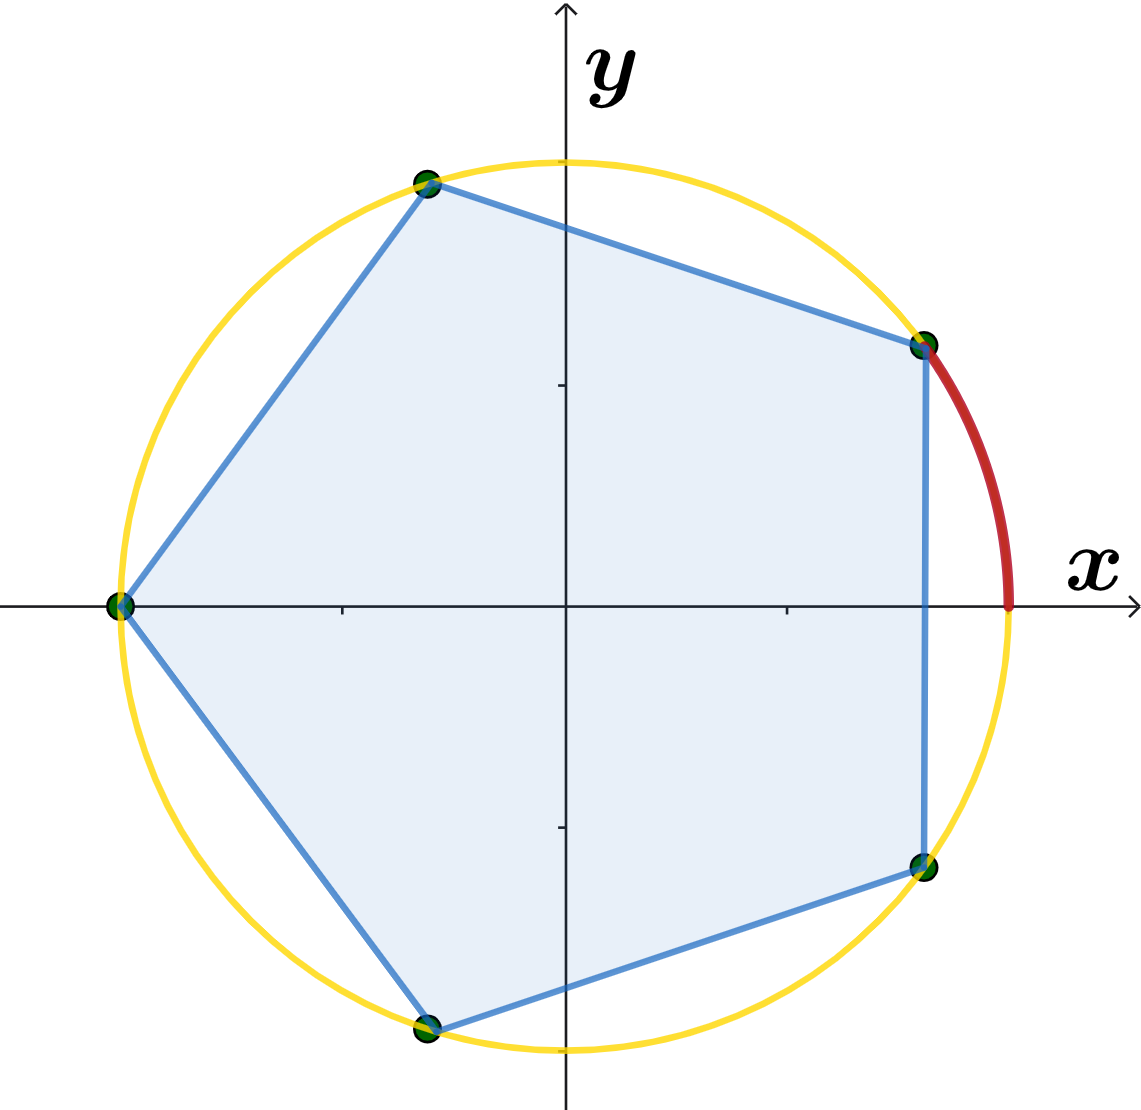
\includegraphics[width=0.35\linewidth]{hipatia pentagono1.png}
    \caption{Projeção no plano $xy$.}
\end{figure}

Os pontos da esfera que são projetados nessa região (aqui contando as partes superior e inferior da esfera que se projetam na região poligonal) formam uma região cuja área pode ser calculada através de $$A = 4\pi - 5 \cdot A_{\mbox{revolução}}$$ onde: $4\pi$ é a área da superfície esférica de raio 1 ($4\pi R^2$), e $A_{\mbox{revolução}}$ é a área da superfície de revolução obtida pela rotação da curva que pode ser parametrizada por $$\mathcal{C} : \begin{cases}
    x(t) = \cos(t), \\ y(t) = \sin(t)
\end{cases} \ \ \ 0 \leq t \leq \frac{\pi}{5}$$ (cujo traço é o arco em destaque na figura), em torno do eixo $x$. Temos que
\begin{align*}
    A_{\mbox{revolução}} &= 2\pi \int_{0}^{\frac{\pi}{5}} y(t)\sqrt{[x'(t)]^2 + [y'(t)]^2} \ dt \\ &= 2\pi \int_{0}^{\frac{\pi}{5}} \sin(t)\sqrt{[-\sin(t)]^2 + [\cos(t)]^2} \ dt \\ &= 2\pi \int_{0}^{\frac{\pi}{5}} \sin(t) \ dt \\ &= 2\pi \left[-\cos(t)\bigg|_{0}^{\pi/5}\right] \\ &= 2\pi(1 - \cos(\pi/5)) = \frac{(3 - \sqrt{5})\pi}{2}
\end{align*}

[O fato de que $\cos(\pi/5) = \frac{1+\sqrt{5}}{4}$ pode ser obtido usando relações trigonométricas em um triângulo isósceles de ângulos $36^{\circ}, 72^{\circ}, 72^{\circ}$ e base 1]. Portanto, $$A = \frac{8\pi - 5(3 - \sqrt{5})\pi}{2} = \frac{(5\sqrt{5} - 7)\pi}{2}.$$









\begin{problem*}
Seja $f$ diferenciável em $x=a$ com $f(a) \neq 0$. Calcule:
$$\displaystyle \lim_{n \to \infty} \left [ \dfrac{f(a+1/n)}{f(a)} \right ]^n.$$
\end{problem*}

\begin{sola}
Basta calcular

\[
\lim_{x \to 0} \left[ \frac{f(a + x)}{f(a)} \right]^{1/x}.
\]

\noindent Como $f$ é contínua, para \( x \) suficientemente pequeno, \( f(a + x) \) e \( f(a) \) têm o mesmo sinal, e daí segue que

$$\log \left[ \lim_{x \to 0} \left( \frac{f(a + x)}{f(a)} \right)^{1/x} \right]
 =  \lim_{x \to 0} \left[ \log \left( \frac{|f(a + x)|}{|f(a)|} \right)^{1/x} \right]$$
$$ =  \lim_{x \to 0} \frac{\log |f(a + x)| - \log |f(a)|}{x}.$$
A última expressão à direita é a definição da derivada de \( \log |f(x)| \) em \( x = a \), que sabemos ser igual a \( f'(a)/f(a) \). Assim,

\[
\lim_{x \to 0} \left[ \frac{f(a + x)}{f(a)} \right]^{1/x} = e^{f'(a)/f(a)}.
\]
\end{sola}






\begin{problem*}
Sejam $A, B \in M(n, \mathbb{C})$ e $P \in \mathbb{C}[X]$ um polinômio não constante tal que $P(0) \neq 0$ e $A B=P(A)$. Prove que a matriz $A$ é invertível e que as matrizes $A$ e $B$ comutam (isto é, que $AB=BA$).
\end{problem*}

\noindent {\textbf{Solução:}} Podemos escrever \( P(X) \) da seguinte forma:
\[
P(X) = P(0) + XQ(X),
\]
onde \( Q \in \mathbb{C}[X] \). Assim segue que
\[
P(A) = P(0) \cdot I_n + AQ(A).
\]
Agora, como \[P(A) = AB, \] temos que \[
AB = P(0) \cdot I_n + AQ(A)\]  e daí $A[B - Q(A)] = P(0)I_n.$
Mas,
\[
P(0) \neq 0
\]
implica que
\[
A \cdot \frac{1}{P(0)}[B - Q(A)] = I_n \implies A^{-1} = \frac{1}{P(0)}[B - Q(A)].
\]

\noindent Logo \( A \) é invertível e a expressão acima é a inversa de \( A \). Por outro lado, \[AB = P(A) \iff B = A^{-1}P(A).\]
Então temos que
\[
BA = A^{-1}P(A)A = A^{-1}AP(A) = I_nP(A) = P(A) = AB.
\]

\noindent Portanto as matrizes \( A \) e \( B \) comutam.




\section{Problemas de Matemática Elementar}

\begin{problem*} O produto dos números reais positivos $a_1, a_2, \ldots, a_n$ é igual a 1. Prove, \textbf{sem ser por indução}, que $$(1+a_1)\cdot(1+a_2)\cdots (1+a_n) \geq 2^n.$$  

\end{problem*}

\noindent \textbf{Solução} (Solução de Vinícius Leite).

\textbf{Desigualdade das Médias (MA-MG)}

A demonstração utiliza a Desigualdade das Médias Aritmética e Geométrica (MA-MG). Para quaisquer números reais positivos $x$ e $y$, temos que
$$\frac{x+y}{2} \ge \sqrt{xy} \implies x+y \ge 2\sqrt{xy}.$$

Aplicando essa desigualdade individualmente para cada par formado por $1$ e $a_i$ (sabendo que $a_i > 0$), construímos o seguinte sistema de desigualdades:
\begin{align*}
    1+a_1 &\ge 2\sqrt{a_1} \\
    1+a_2 &\ge 2\sqrt{a_2} \\
    &\ \ \vdots \\
    1+a_n &\ge 2\sqrt{a_n}.
\end{align*}

Como todos os termos em ambos os lados das desigualdades são estritamente positivos, podemos multiplicar as $n$ desigualdades membro a membro sem alterar o sentido da relação:
$$(1+a_1)(1+a_2)\cdots(1+a_n) \ge (2\sqrt{a_1})(2\sqrt{a_2})\cdots(2\sqrt{a_n}).$$

Agrupando os $n$ fatores $2$ e unificando as raízes no lado direito, obtemos
$$(1+a_1)(1+a_2)\cdots(1+a_n) \ge 2^n\sqrt{a_1\cdot a_2 \cdots a_n}.$$

Por hipótese, o produto de todos os termos $a_i$ é exatamente 1 ($a_1\cdot a_2 \cdots a_n = 1$). Substituindo esse valor, a expressão sob a raiz resulta em 1 (elemento neutro da multiplicação):
$$(1+a_1)(1+a_2)\cdots(1+a_n) \ge 2^n\sqrt{1}.$$

O que demonstra diretamente a tese:
$$(1+a_1)(1+a_2)\cdots(1+a_n) \ge 2^n.$$



\begin{problem*} Seja $A$ um subconjunto dos números naturais tal que, entre 100 números naturais consecutivos, existe um elemento de $A$. Prove que podemos encontrar quatro números diferentes $a, b, c$ e $d$ em $A$ tais que $a+b = c+d$.  

\end{problem*}

\noindent \textbf{Solução} (Solução de Victor Leite). 

\textbf{1\superou  Passo: A infinitude do conjunto $A$}

Dado que entre 100 naturais consecutivos existe, ao menos, um elemento de $A$, podemos concluir que o número de elementos de $A$ equivale, no mínimo, à quantidade de partições de 100 elementos do conjunto dos naturais, que por sua vez é infinito. Logo, podemos afirmar que o conjunto $A$ possui infinitos termos.

\vspace{0.5cm}
\textbf{2\superou  Passo: O Princípio da Casa dos Pombos}

Provar que $\exists \ a, b, c, d \in A \mid a+b = c+d$ equivale a provar que para $a, b, c, d \in A$, $a-c = d-b$, o que, por sua vez, equivale a provar que a distância entre $a$ e $c$ equivale à distância entre $d$ e $b$.

Sabendo que a cada 100 naturais consecutivos existe sempre ao menos um elemento de $A$, podemos afirmar que em qualquer intervalo fechado do tipo $[a_n, a_n+100]$ existirão ao menos 2 elementos de $A$. Logo, a distância máxima possível entre dois elementos consecutivos $a_n$ e $a_{n+1}$ pertencentes ao conjunto $A$ é rigorosamente 100.

Como as distâncias entre elementos consecutivos resultam em números inteiros, todas as distâncias possíveis pertencem ao intervalo $[1, 100]$. Portanto, o número máximo de distâncias distintas entre elementos consecutivos de $A$ é 100.

Para aplicar o Princípio da Casa dos Pombos, analisamos os 202 primeiros elementos de $A$. Com eles, podemos formar exatamente 101 pares disjuntos de elementos consecutivos:
$$(a_1, a_2), (a_3, a_4), \dots, (a_{201}, a_{202}).$$

Temos 101 pares gerando 101 medidas de distância. Como existem no máximo 100 valores distintos possíveis para essas distâncias, o Princípio da Casa dos Pombos (Teorema de Dirichlet) garante que, inevitavelmente, ao menos 2 pares disjuntos possuirão exatamente a mesma distância.

Sejam esses pares disjuntos $(c, a)$ e $(b, d)$, ambos pertencentes a $A$, tais que a distância do primeiro par seja igual à distância do segundo par:
$$a - c = d - b.$$

Manipulando algebricamente a igualdade, obtemos diretamente:
$$a + b = c + d.$$

Como os dois pares analisados são disjuntos e os elementos de $A$ podem ser dispostos em uma sequência estritamente crescente de naturais, os quatro números $a, b, c$ e $d$ são obrigatoriamente distintos, o que conclui a prova.
















\begin{problem*} Uma pilha tem 40 pedras. A pilha é dividida em duas partes, depois uma das partes é dividida em duas novamente, etc., até termos 40 pedras separadas (40 pilhas formadas com uma pedra cada). Depois de cada divisão de uma das pilhas em duas menores, escrevemos o produto dos números de pedras nestas duas pilhas em um quadro. Mostre que, no final, a soma de todos os números no quadro será igual a 780. 

\end{problem*}

\noindent \textbf{Solução:}
Para mostrar o resultado desejado, vamos analisar o problema de um ponto de vista mais geral, para tentar achar algum padrão que possa ser generalizado e então resolver o caso particular de $40$ pedras. Seja $n$ o número de pedras no início da divisão e chamemos de $S_n$ a soma final obtida ao final do processo. 

\begin{itemize}

\item Para $n = 2$: a única opção de divisão é $2 = 1 + 1$, cujo produto é $S_2 = 1$;

\item Para $n = 3$: por simetria, podemos considerar a divisão inicial $3 = 2 + 1$, anotando no quadro o valor $2$. Após isso, veja que os próximos números a serem anotados no quadro são os que podem ser gerados começando com $2$ pedras. Nesse caso, já sabemos o que ocorre. Assim, ao final teremos a soma $S_3 = 2 + 1 = 3$;

\item Para $n = 4$: podemos começar com duas possíveis divisões iniciais $4 = 2 + 2$ ou $4 = 3 + 1$, anotando no quadro o valor $4$ ou $3$, respectivamente. Após isso, veja que os próximos números a serem anotados no quadro são os que podem ser gerados começando com $2$ pedras ou $3$ pedras. Nesse caso, já sabemos o que ocorre. Assim, ao final teremos a soma $S_4 = 4 + 1 + 1 = 6$ (no primeiro caso) e $S_4 = 3 + 3 = 6$ (no segundo caso). Podemos ver que, de fato, a soma final $S_n$ parece não depender das escolhas de divisões feitas;

\item Suponha que esse padrão de independência das escolhas de divisões não afete a soma final. Ao começar com $n$ pedras, façamos a divisão $n = (n - 1) + 1$, anotando o produto $n - 1$. Sucedendo nesse padrão de divisão, sempre separando apenas 1 pedra em cada etapa, teremos anotado os produtos $n - 1, \ n - 2, \ldots, 2$ e $1$, cuja soma é $S_n = \frac{n(n-1)}{2}$.
\end{itemize}

Pronto, agora vamos provar em definitivo que, de fato, isso independe das escolhas de divisões iniciais e intermediárias. Provaremos, por indução, que $S_n = \frac{n(n-1)}{2}$ independe das escolhas de divisões. 

\ 

Para $n = 2$, já temos o desejado. Agora, suponhamos que isso vale para todo $k$ natural entre $2$ e $n - 1$, isto é, que $S_k = \frac{k(k-1)}{2}$ independe das escolhas de divisões, $k = 2, \ldots, n - 1$. 

\ 

Agora, partindo de $n$ pedras, podemos fazer a divisão inicial $n = k + (n - k)$ com $k, n - k \leq n - 1$. Temos que o produto inicial anotado no quadro é $k(n - k)$. Mas, por hipótese de indução, vale que $S_k = \frac{k(k-1)}{2}$ e $S_{n-k} = \frac{(n-k)(n-k-1)}{2}$ (aqui supondo que $S_1 = 0$). Assim, a soma dos produtos anotados no quadro é 
$$k(n - k) + \frac{k(k-1)}{2} + \frac{(n-k)(n-k-1)}{2} $$
$$= \frac{2k(n-k) + k^2 + (n-k)^2 - k - (n-k)}{2}$$ 
$$= \frac{(k + (n-k))^2 - n}{2} = \frac{n^2 - n}{2} = \frac{n(n-1)}{2}.$$ Portanto, $S_n = \frac{n(n-1)}{2}$, e o resultado vale para todo $n \geq 2$ ($n \geq 1$ se incluirmos $S_1 = 0$). Com isso, $S_{40} = \frac{40 \cdot 39}{2} = 780$, como queríamos demonstrar.







\begin{problem*}
A sequência de números inteiros $x_n$ é definida por $x_1 = 4$, $x_2 = 6$ e, para $n \geq 3$, $x_n$ é o menor número composto maior que $2x_{n-1} - x_{n-2}$. Encontre o valor de $x_{2026}$.
\end{problem*}

\noindent \textbf{Solução:}

\noindent Vamos calcular os primeiros termos da sequência:

\begin{eqnarray*}
2x_{2} - x_1 = 8 & \Rightarrow & x_3 = 9 \\
2x_{3} - x_2 = 12 & \Rightarrow & x_4 = 14 \\
2x_{4} - x_3 = 19 & \Rightarrow & x_5 = 20 \\
2x_{5} - x_4 = 26 & \Rightarrow & x_6 = 27 .\\
\end{eqnarray*}

\noindent Note que 

\begin{eqnarray*}
x_4 - x_3 & = & 5 \\
x_5 - x_4 & = & 6 \\
x_6 - x_5 & = & 7 .\\
\end{eqnarray*}

\noindent Isso nos permite conjecturar que 

$$x_{n} - x_{n-1} = n + 1.$$

\noindent Realizando a soma telescópica da identidade anterior para $n \in \{4,5, \ldots, k\}$, obtemos 
\begin{eqnarray*}
x_i & = & x_3 + 5 + 6 + \ldots + (i+1) \\
	& = & \dfrac{i(i+3)}{2}. 
\end{eqnarray*}

Provemos a afirmação anterior por indução. Suponha que ela vale para todos os inteiros $i \in \{3,4, \ldots, k\}$. Para provar que também vale para $k+1$, note que 

$$2x_k - x_{k-1} = 2 \cdot \dfrac{k(k+3)}{2} - \dfrac{(k-1)(k+2)}{2} = \dfrac{(k+1)(k+4)}{2} - 1.$$
Se $k \geq 3$, a depender da paridade de $k$, podemos escrever $\dfrac{(k+1)(k+4)}{2} = \dfrac{k+1}{2} \cdot (k+4)$ ou $\dfrac{k+4}{2} \cdot (k+1)$, garantindo assim que 
$$x_{k+1} = \dfrac{(k+1)(k+4)}{2}.$$
Portanto, $x_{2026} = \dfrac{2026 \cdot 2029}{2}.$

\begin{problem*}
Em uma festa, existem $25$ membros que satisfazem a seguinte condição: quando dois deles não se conhecem, então eles possuem algum amigo em comum. Sabemos que ninguém conhece todos na festa. Prove que a soma dos números de amigos de cada pessoa na festa é pelo menos $72$.
\end{problem*}

\noindent \textbf{Solução:}

Primeiramente observe que se uma pessoa da festa conhecer apenas uma outra, então essa última será obrigada a conhecer todos os demais da festa. Portanto, todos na festa conhecem pelo menos duas pessoas. Suponha, por absurdo, que a soma dos números de amigos de cada um é menor que $72$. Como ela deve ser um número par, ela é no máximo $70$. Dado que $70/3 < 25$, pelo Princípio da Casa dos Pombos, há uma pessoa, digamos $A$, que conhece exatamente duas outras pessoas, digamos $B$ e $C$. As outras $22$ pessoas que não conhecem $A$ obrigatoriamente devem conhecer $B$ ou $C$. Assim, a soma dos números de amigos de $A$, $B$ e $C$ é pelo menos $2+1+1+22 = 26$. Cada uma das outras $22$ pessoas conhece pelo menos duas outras, e assim a soma dos números de amigos de todos é pelo menos $22\cdot 2 + 26 = 70$. Para que ocorra essa igualdade, $B$ e $C$ não devem se conhecer, e cada um dos demais membros deve conhecer exatamente um dos dois. Isso nos permite classificar os $22$ membros que não estão em $\{A,B,C\}$ em dois grupos: o grupo $G_B$ (dos que conhecem $B$) e o grupo $G_C$ (dos que conhecem $C$). Pelo Princípio da Casa dos Pombos, pelo menos um desses grupos, digamos $G_B$, possui $11$ membros. Se $C$ conhecer qualquer um deles, a soma anterior irá ultrapassar $70$. Para que isso não ocorra, $C$ deve possuir um amigo em comum com cada um dos membros de $G_B$, que necessariamente devem ser distintos, porque cada um deles conhece apenas $2$ pessoas. Consequentemente, $G_C$ possui pelo menos $11$ membros. Isso é um absurdo, porque uma pessoa de $G_B$ que não conheça uma de $G_C$ não poderá ter um amigo em comum com ela.

\begin{problem*}
Seja $ABCD$ um quadrilátero inscritível e $P=BD \cap AC$. Os pés das perpendiculares de $P$ aos lados $AB$ e $CD$ são $X$ e $Y$. Se $M$ e $N$ são os pontos médios dos lados $BC$ e $AD$, prove que $MN \perp XY$.    
\end{problem*}



\noindent \textbf{Solução} (Solução de Roberto Sant'anna e Yan Lima Machado) 

Pelo enunciado, tem-se o seguinte esboço:
\vspace*{0.2cm}

\begin{tikzpicture}[
    scale=1.2,
    angle/.style={draw, angle radius=0.5cm, angle eccentricity=1.6}
]

    % 1. Coordenadas principais 
    % (Raio fixo = 3 garante que todos estão na mesma circunferência, ou seja, é inscritível.)
    \coordinate (A) at (190:3);
    \coordinate (B) at (350:3);
    \coordinate (C) at (60:3);  % Assimétrico para não parecer trapézio
    \coordinate (D) at (110:3); % Assimétrico para não parecer trapézio

    % 2. Interseção das diagonais (Ponto P)
    \path[name path=AC] (A) -- (C);
    \path[name path=BD] (B) -- (D);
    \path [name intersections={of=AC and BD, by=P}];

    % 3. Pés das perpendiculares (X e Y)
    \coordinate (X) at ($(A)!(P)!(B)$);
    \coordinate (Y) at ($(C)!(P)!(D)$);

    % 4. Pontos médios (M e N)
    \coordinate (N) at ($(A)!0.5!(D)$);
    \coordinate (M) at ($(B)!0.5!(C)$);

    % 5. Desenhando as linhas do quadrilátero e diagonais
    \draw[thick, blue] (A) -- (B) -- (C) -- (D) -- cycle;
    \draw[thick, red] (A) -- (C);
    \draw[thick, red] (B) -- (D);

    % 6. Desenhando as linhas tracejadas
    \draw[dashed, thick] (X) -- (P);
    \draw[dashed, thick] (P) -- (Y);
    \draw[dashed, thick] (N) -- (P);
    \draw[dashed, thick] (P) -- (M);

    % 7. Marcações de ângulo reto em X e Y com o pontinho centralizado
    \pic [draw, gray, thick, angle radius=3mm] {right angle = P--X--B};
    \coordinate (dotX) at ($(X)!0.8mm!(P) + ($(X)!0.8mm!(B) - (X)$)$);
    \fill[gray] (dotX) circle (0.4pt);

    \pic [draw, gray, thick, angle radius=3mm] {right angle = P--Y--D};
    \coordinate (dotY) at ($(Y)!0.8mm!(P) + ($(Y)!0.8mm!(D) - (Y)$)$);
    \fill[gray] (dotY) circle (0.4pt);

    % 8. Rótulos dos vértices e pontos
    \node[below left, text=purple] at (A) {A};
    \node[below right, text=purple] at (B) {B};
    \node[above right, text=purple] at (C) {C};
    \node[above left, text=purple] at (D) {D};
    \node[above, text=purple, yshift=5mm, xshift=-2mm] at (P) {P};
    \node[below, text=purple, yshift=-1mm] at (X) {X};
    \node[above, text=purple, yshift=1mm] at (Y) {Y};
    \node[left, text=purple, xshift=-1mm] at (N) {N};
    \node[right, text=purple, xshift=1mm] at (M) {M};

    % 9. Ângulos internos nas quinas

    \pic [draw, text=blue, angle eccentricity=1.6, "$\alpha$"] {angle = B--A--C};
    \pic [draw, text=blue, angle eccentricity=1.6, "$\alpha$"] {angle = B--D--C};
    
    \pic [draw, text=blue, angle eccentricity=1.6, "$\beta$"] {angle = D--C--A};
    \pic [draw, angle eccentricity=1.6, "$\beta$"] {angle = D--B--A};

    \pic [draw, text=blue, angle eccentricity=1.6, "$\gamma$"] {angle = A--D--C};
    \pic [draw, text=blue, angle eccentricity=1.6, "$\gamma$"] {angle = A--C--B};
    
    \pic [draw, text=blue, angle eccentricity=1.6, "$\lambda$"] {angle = C--A--D};
    \pic [draw, text=blue, angle eccentricity=1.6, "$\lambda$"] {angle = C--B--D};

    % 10. Ângulos centrais no ponto P usando a biblioteca
    \pic [draw, thick, green!50!black, angle radius=4mm] {angle = A--P--X};
    \pic [draw, thick, green!50!black, angle radius=4mm] {angle = Y--P--D};
    
    \pic [draw, thick, cyan, angle radius=4mm] {angle = X--P--B};
    \pic [draw, thick, cyan, angle radius=4mm] {angle = C--P--Y};

    % 11. Marcações de congruência nos pontos médios
    \coordinate (Nup) at ($(N)!8mm!(D)$);
    \coordinate (Ndown) at ($(N)!7mm!(A)$);
    \draw[thick] ($(Nup)!1.5mm!90:(A)$) -- ($(Nup)!-1.5mm!90:(A)$);
    \draw[thick] ($(Ndown)!1.5mm!90:(A)$) -- ($(Ndown)!-1.5mm!90:(A)$);
    
    \coordinate (Mup1) at ($(M)!8mm!(C)$);
    \coordinate (Mdown1) at ($(M)!7mm!(C)$);
    \draw[thick] ($(Mup1)!1.5mm!90:(B)$) -- ($(Mup1)!-1.5mm!90:(B)$);
    \draw[thick] ($(Mdown1)!1.5mm!90:(B)$) -- ($(Mdown1)!-1.5mm!90:(B)$);

    \coordinate (Mup2) at ($(M)!7mm!(B)$);
    \coordinate (Mdown2) at ($(M)!6mm!(B)$);
    \draw[thick] ($(Mup2)!1.5mm!90:(B)$) -- ($(Mup2)!-1.5mm!90:(B)$);
    \draw[thick] ($(Mdown2)!1.5mm!90:(B)$) -- ($(Mdown2)!-1.5mm!90:(B)$);

\end{tikzpicture}

\vspace*{0.5cm}

Como $ABCD$ é inscritível, tem-se que $\angle BDC = \angle CAB = \alpha$, $\angle DBA = \angle DCA = \beta$, $\angle ADB = \angle ACB = \gamma$ e $\angle DAC = \angle DBC = \lambda$. Ademais, tem-se que $PX$ e $PY$ são alturas dos triângulos $ABP$ e $CDP$, respectivamente. 

\vspace*{0.2cm}

Portanto, tem-se que os triângulos $CDP$ e $ABP$ são semelhantes e, daí, tem-se que:

\vspace*{0.2cm}

\begin{center}
$\dfrac{AB}{CD}=\dfrac{XP}{YP}$.
\end{center}

\vspace{0.2cm}

Seja $E$ o ponto médio de $AC$ (esboço abaixo). Como $M$ e $N$ são pontos médios de $AD$ e $BC$ respectivamente, temos que $EM$ é base média de $ABC$ e, portanto

\vspace*{0.2cm}

\begin{center}
$\dfrac{AB}{CD}=\dfrac{EM}{EN}=\dfrac{XP}{YP}$ (1). 
\end{center}


\begin{tikzpicture}[
    scale=1.2,
    angle/.style={draw, angle radius=0.5cm, angle eccentricity=1.6}
]

    % 1. Coordenadas principais 
    % (Raio fixo = 3 garante que todos estão na mesma circunferência, ou seja, é inscritível.)
    \coordinate (A) at (190:3);
    \coordinate (B) at (350:3);
    \coordinate (C) at (60:3);  % Assimétrico para não parecer trapézio
    \coordinate (D) at (110:3); % Assimétrico para não parecer trapézio

    % 2. Interseção das diagonais (Ponto P)
    \path[name path=AC] (A) -- (C);
    \path[name path=BD] (B) -- (D);
    \path [name intersections={of=AC and BD, by=P}];

    % 3. Pés das perpendiculares (X e Y)
    \coordinate (X) at ($(A)!(P)!(B)$);
    \coordinate (Y) at ($(C)!(P)!(D)$);

    % 4. Pontos médios (M, N e E)
    \coordinate (N) at ($(A)!0.5!(D)$);
    \coordinate (M) at ($(B)!0.5!(C)$);
    \coordinate (E) at ($(A)!0.5!(C)$); % ponto médio de AC

    % 5. Desenhando as linhas do quadrilátero e diagonais
    \draw[thick, blue] (A) -- (B) -- (C) -- (D) -- cycle;
    \draw[thick, red] (A) -- (C);
    \draw[thick, red] (B) -- (D);

   % 6. Desenhando as linhas tracejadas
    \draw[dashed, thick] (X) -- (P);
    \draw[dashed, thick] (P) -- (Y);
    \draw[dashed, thick] (N) -- (P);
    \draw[dashed, thick] (P) -- (M);

    % Segmentos EM e EN
    \draw[green, thick] (E) -- (M);
    \draw[yellow, thick] (E) -- (N);

    % 7. Marcações de ângulo reto em X e Y com o pontinho centralizado
    \pic [draw, gray, thick, angle radius=3mm] {right angle = P--X--B};
    \coordinate (dotX) at ($(X)!0.8mm!(P) + ($(X)!0.8mm!(B) - (X)$)$);
    \fill[gray] (dotX) circle (0.4pt);

    \pic [draw, gray, thick, angle radius=3mm] {right angle = P--Y--D};
    \coordinate (dotY) at ($(Y)!0.8mm!(P) + ($(Y)!0.8mm!(D) - (Y)$)$);
    \fill[gray] (dotY) circle (0.4pt);

    % 8. Rótulos dos vértices e pontos
    \fill (E) circle (1.2pt);

    \node[below left, text=purple] at (A) {A};
    \node[below right, text=purple] at (B) {B};
    \node[above right, text=purple] at (C) {C};
    \node[above left, text=purple] at (D) {D};
    \node[above, text=purple, yshift=5mm, xshift=-2mm] at (P) {P};
    \node[below, text=purple, yshift=-1mm] at (X) {X};
    \node[above, text=purple, yshift=1mm] at (Y) {Y};
    \node[left, text=purple, xshift=-1mm] at (N) {N};
    \node[right, text=purple, xshift=1mm] at (M) {M};
    \node[right, text=purple, xshift=1mm] at (E) {E};

    % 9. Ângulos internos nas quinas
    \pic [draw, text=blue, angle eccentricity=1.6, "$\alpha$"] {angle = B--A--C};
    \pic [draw, text=blue, angle eccentricity=1.6, "$\alpha$"] {angle = B--D--C};
    
    \pic [draw, text=blue, angle eccentricity=1.6, "$\beta$"] {angle = D--C--A};
    \pic [draw, text=blue, angle eccentricity=1.6, "$\beta$"] {angle = D--B--A};

    \pic [draw, text=blue, angle eccentricity=1.6, "$\gamma$"] {angle = A--D--C};
    \pic [draw, text=blue, angle eccentricity=1.6, "$\gamma$"] {angle = A--C--B};
    
    \pic [draw, text=blue, angle eccentricity=1.6, "$\lambda$"] {angle = C--A--D};
    \pic [draw, text=blue, angle eccentricity=1.6, "$\lambda$"] {angle = C--B--D};

    % 10. Ângulos centrais no ponto P usando a biblioteca
    \pic [draw, thick, green!50!black, angle radius=4mm] {angle = A--P--X};
    \pic [draw, thick, green!50!black, angle radius=4mm] {angle = Y--P--D};
    
    \pic [draw, thick, cyan, angle radius=4mm] {angle = X--P--B};
    \pic [draw, thick, cyan, angle radius=4mm] {angle = C--P--Y};

    % 11. Marcações de congruência nos pontos médios
    \coordinate (Nup) at ($(N)!8mm!(D)$);
    \coordinate (Ndown) at ($(N)!7mm!(A)$);
    \draw[thick] ($(Nup)!1.5mm!90:(A)$) -- ($(Nup)!-1.5mm!90:(A)$);
    \draw[thick] ($(Ndown)!1.5mm!90:(A)$) -- ($(Ndown)!-1.5mm!90:(A)$);
    
    \coordinate (Mup1) at ($(M)!8mm!(C)$);
    \coordinate (Mdown1) at ($(M)!7mm!(C)$);
    \draw[thick] ($(Mup1)!1.5mm!90:(B)$) -- ($(Mup1)!-1.5mm!90:(B)$);
    \draw[thick] ($(Mdown1)!1.5mm!90:(B)$) -- ($(Mdown1)!-1.5mm!90:(B)$);

    \coordinate (Mup2) at ($(M)!7mm!(B)$);
    \coordinate (Mdown2) at ($(M)!6mm!(B)$);
    \draw[thick] ($(Mup2)!1.5mm!90:(B)$) -- ($(Mup2)!-1.5mm!90:(B)$);
    \draw[thick] ($(Mdown2)!1.5mm!90:(B)$) -- ($(Mdown2)!-1.5mm!90:(B)$);

\end{tikzpicture}

\vspace{0.2cm}

Ademais, $EM \parallel AB$ e $EN \parallel CD$.

\vspace{0.2cm}

Pela conclusão anterior, sem perda de generalidade, pode-se inferir que $PX$ é perpendicular à reta suporte de $EM$, chamemo-la de $r$. Analogamente, $PY$ é perpendicular à reta suporte de $EN$, chamemo-la de $s$.

\vspace{0.2cm}

Analisando os ângulos $\angle NEM$ e $\angle YPX$, tem-se que ambos são congruentes.

\vspace{0.3cm}

\textbf{Prova}: Como $EM \parallel AB$ e $EN \parallel CD$, ao prolongar os lados AB e CD, eles se encontram num ponto F, o ângulo obtuso formado entre os prolongamentos é congruente ao ângulo $\angle NEM$.

\vspace{0.2cm}

\begin{tikzpicture}[
    scale=0.6   ,
    angle/.style={draw, angle radius=0.5cm, angle eccentricity=1.6}
]

    % 1. Coordenadas principais do quadrilátero genérico
    \coordinate (A) at (190:3);
    \coordinate (B) at (350:3);
    \coordinate (C) at (40:3);
    \coordinate (D) at (90:3);

    % 2. Ponto F: Interseção dos prolongamentos
    \coordinate (F) at (intersection of A--B and D--C);
    
    % Pontos auxiliares para prolongar as retas um pouco ALÉM de F
    \coordinate (FextAB) at ($(A)!1.2!(F)$);
    \coordinate (FextDC) at ($(D)!1.2!(F)$);

    % 3. Interseção das diagonais (Ponto P)
    \path[name path=AC] (A) -- (C);
    \path[name path=BD] (B) -- (D);
    \path [name intersections={of=AC and BD, by=P}];

    % 4. Pés das perpendiculares (X e Y)
    \coordinate (X) at ($(A)!(P)!(B)$);
    \coordinate (Y) at ($(C)!(P)!(D)$);

    % 5. Pontos médios N(em AD), M(em BC) e o NOVO ponto E(em AC)
    \coordinate (N) at ($(A)!0.5!(D)$);
    \coordinate (M) at ($(B)!0.5!(C)$);
    \coordinate (E) at ($(A)!0.5!(C)$); % Base média

    % 6. Desenhando as linhas do quadrilátero e diagonais
    \draw[thick, blue] (A) -- (B) -- (C) -- (D) -- cycle;
    \draw[thick, red] (A) -- (C);
    \draw[thick, red] (B) -- (D);

    % 7. Desenhando as bases médias (EM e EN) em verde
    \draw[thick, green!60!black] (E) -- (M);
    \draw[thick, green!60!black] (E) -- (N);

    % 8. Prolongamentos passando por F (Tracejado cinza)
    \draw[dashed, thick, gray] (B) -- (FextAB);
    \draw[dashed, thick, gray] (C) -- (FextDC);

    % 9. Desenhando as linhas de X e Y até P e o segmento MN
    \draw[dashed, thick] (X) -- (P);
    \draw[dashed, thick] (P) -- (Y);
    \draw[dashed, thick] (N) -- (M); 

    % 10. Marcações de ângulo reto em X e Y
    \pic [draw, gray, thick, angle radius=3mm] {right angle = P--X--B};
    \coordinate (dotX) at ($(X)!0.8mm!(P) + ($(X)!0.8mm!(B) - (X)$)$);
    \fill[gray] (dotX) circle (0.4pt);

    \pic [draw, gray, thick, angle radius=3mm] {right angle = P--Y--D};
    \coordinate (dotY) at ($(Y)!0.8mm!(P) + ($(Y)!0.8mm!(D) - (Y)$)$);
    \fill[gray] (dotY) circle (0.4pt);

    % 11. MARCAÇÕES DE CONGRUÊNCIA
    % Lado AD (1 traço indicando que N é ponto médio)
    \coordinate (N1) at ($(N)!11mm!(D)$);
    \coordinate (N2) at ($(N)!11mm!(A)$);
    \draw[thick] ($(N1)!1.5mm!90:(A)$) -- ($(N1)!-1.5mm!90:(A)$);
    \draw[thick] ($(N2)!1.5mm!90:(A)$) -- ($(N2)!-1.5mm!90:(A)$);
    
    % Lado BC (2 traços indicando que M é ponto médio)
    \coordinate (M1a) at ($(M)!6mm!(C)$);
    \coordinate (M1b) at ($(M)!5.5mm!(C)$);
    \draw[thick] ($(M1a)!1.5mm!90:(B)$) -- ($(M1a)!-1.5mm!90:(B)$);
    \draw[thick] ($(M1b)!1.5mm!90:(B)$) -- ($(M1b)!-1.5mm!90:(B)$);
    
    \coordinate (M2a) at ($(M)!6mm!(B)$);
    \coordinate (M2b) at ($(M)!5.5mm!(B)$);
    \draw[thick] ($(M2a)!1.5mm!90:(B)$) -- ($(M2a)!-1.5mm!90:(B)$);
    \draw[thick] ($(M2b)!1.5mm!90:(B)$) -- ($(M2b)!-1.5mm!90:(B)$);

    % 12. ÂNGULOS (Destacando a congruência LAL)
    % Ângulo interno na base média (Amarelo)
    \pic [draw, thick, fill=yellow!30, angle radius=4mm] {angle = M--E--N};
    
    % Ângulo Obtuso em F (Amarelo - Correspondente ao MEN)
    \pic [draw, thick, fill=yellow!30, angle radius=4mm] {angle = FextAB--F--C};
    
    % Ângulo Agudo em F (Azul claro - Apenas para referência)
    \pic [draw, thick, fill=cyan!15, angle radius=4mm] {angle = C--F--B};

    % 13. Rótulos dos vértices e pontos
    \node[left, text=purple] at (A) {A};
    \node[below right, text=purple] at (B) {B};
    \node[above right, text=purple] at (C) {C};
    \node[above left, text=purple] at (D) {D};
    \node[above right, text=black, xshift=-2mm, yshift=-5mm] at (F) {F}; % Rótulo de F
    \node[above, text=purple, yshift=5mm, xshift=-2mm] at (P) {P};
    \node[below, text=purple, yshift=-1mm] at (X) {X};
    \node[above right, text=purple, xshift=1mm, yshift=1mm] at (Y) {Y};
    \node[above left, text=purple, xshift=-1mm] at (N) {N};
    \node[right, text=purple, xshift=1mm] at (M) {M};
    \node[below, text=green!60!black, yshift=-1mm] at (E) {E}; % Rótulo de E

\end{tikzpicture}

\vspace{0.3cm}

Analisando o quadrilátero $FYPX$ formado, tem-se, na soma dos ângulos internos, que:

\vspace{0.2cm}

\begin{center}
$\angle XFY + 90^o + 90^o + \angle YPX = 360^o$
\end{center}

\vspace{0.2cm}

\begin{center}
$\Leftrightarrow \angle YPX = 180^o - \angle XFY$
\end{center}

\vspace{0.05cm}

\begin{center}
$\Leftrightarrow \angle YPX = \angle NEM$ (2)
\end{center}

\vspace{0.2cm}

Logo, pelas equações (1) e (2), tem-se que $NEM$ e $XYP$ são triângulos semelhantes devido ao caso LAL de semelhança.

\vspace{0.2cm}

Como visto anteriormente, $PX \perp r \supset EM$ e $PY \perp s \supset EN$; então, obrigatoriamente, $MN \perp XY$. Isso é comprovado pelo fato de que a relação de semelhança consiste em realizar, no máximo, rotações e translações. Assim, ao realizar algum desses movimentos de tal forma que dois pares de lados homólogos sejam perpendiculares entre si, então o terceiro par também será perpendicular.

\vspace{1cm}

\noindent \textbf{Solução} (solução oficial).

\begin{figure}[htb!]
	\centering
		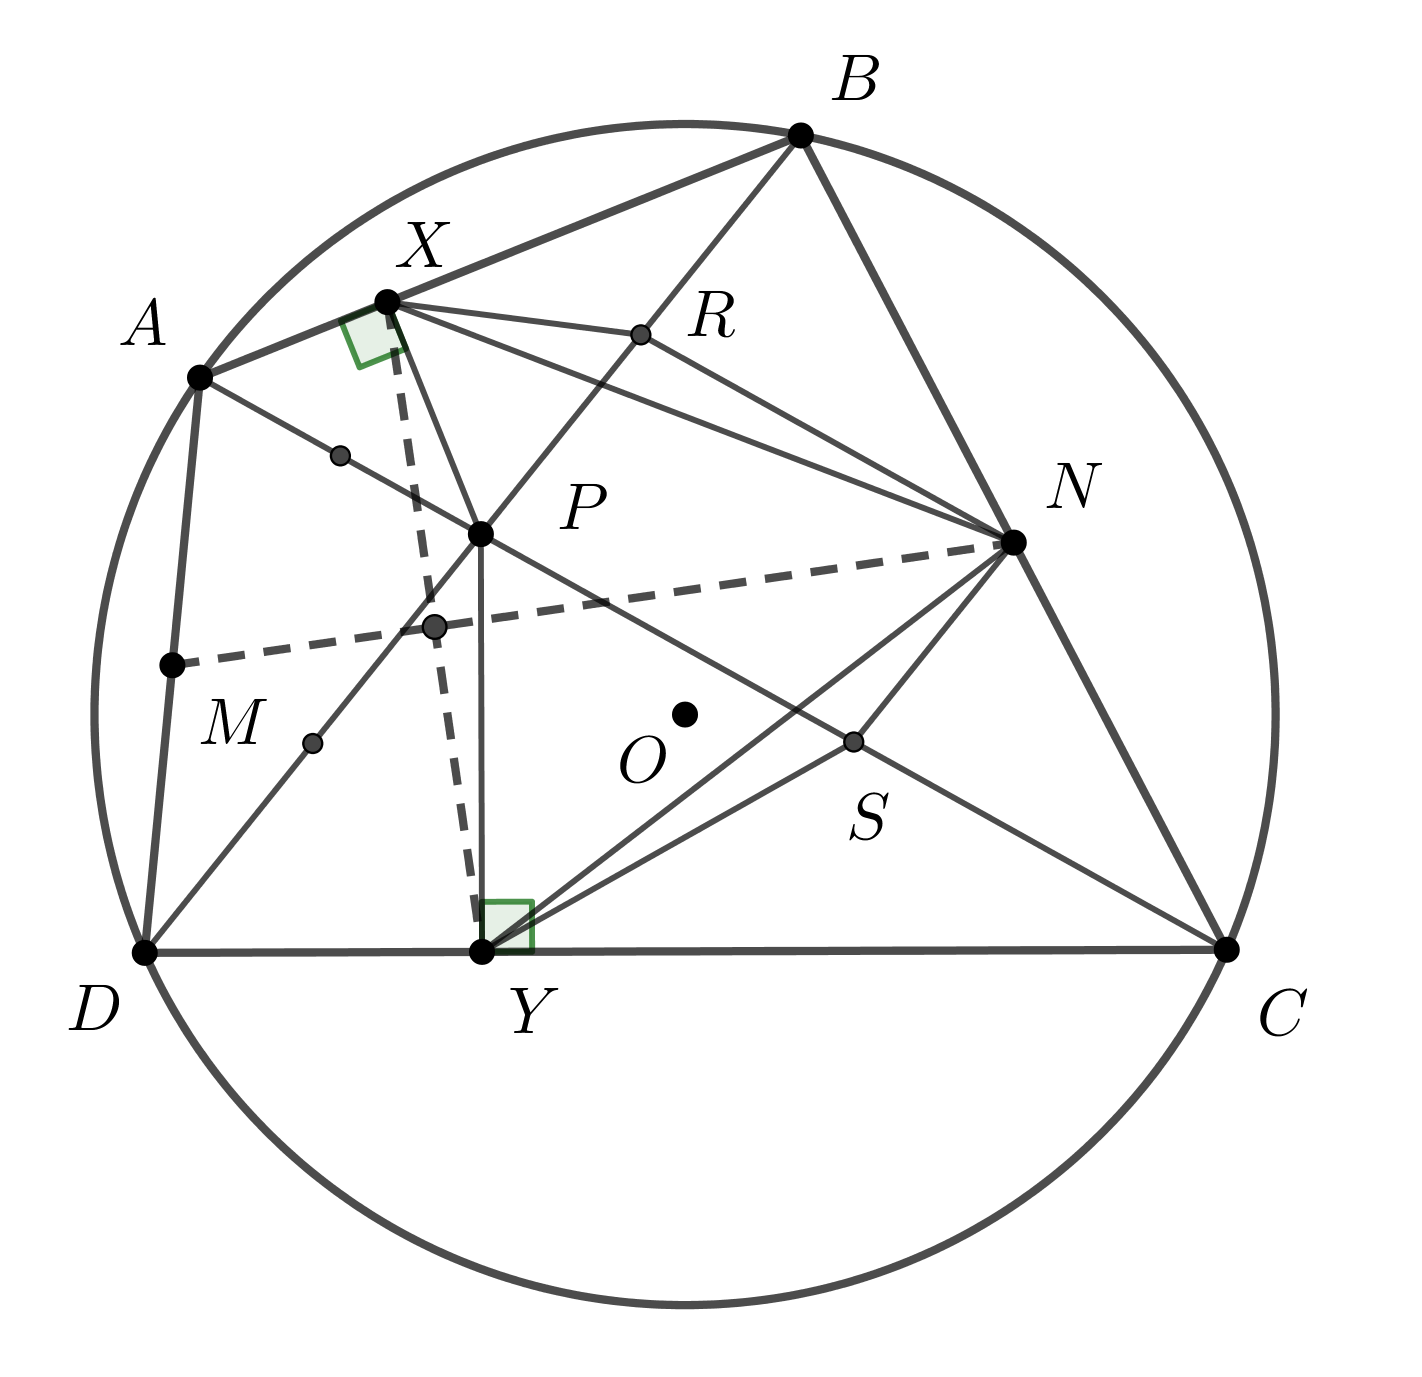
\includegraphics[scale=0.4]{W2.png}
\end{figure}

\noindent Sejam $R$ e $S$ os pontos médios de $BP$ e $CP$, respectivamente. Os triângulos $XRN$ e $NSY$ são congruentes pelo caso $LAL$. Daí $XN=NY$. De forma análoga, $MX=MY$. Portanto, $MN$ é a mediatriz de $XY$.


\begin{problem*}
    Uma máquina tem dois botões: um deles dobra um número inteiro e o outro o aumenta em $1$ unidade. Por exemplo, apertando os botões dessa máquina é possível realizar as seguintes operações:

$$1 \rightarrow_{+1} 2 \rightarrow_{\times 2} 4 \rightarrow_{+1} 5.$$

\noindent Se no início você começa com o número $0$, qual é o número mínimo de vezes que você precisa apertar botões dessa máquina para obter:
\begin{enumerate}[a)]
\item $100$?
\item $2024$?
\end{enumerate} 
\end{problem*}

\noindent \textbf{Solução:}

\noindent Podemos considerar o problema reverso de transformar o número inteiro $n$ em $0$ por meio de duas operações: dividir por $2$ ou subtrair $1$. Seja $r(n)$ o número mínimo de movimentos para transformar $n$ em $0$ com essas duas operações. Claramente, $r(2n+1) = r(2n) + 1$, pois não podemos dividir por $2$. Vamos provar por indução que $r(2k) = 1 + r(k)$. Para $k = 1$ é imediato. Suponha que já provamos para todos os números pares menores que $2k$. Se aplicarmos a operação de subtrair $1$ de $2k$, o número mínimo de operações para obter $0$ não será menor que $1 + r(2k-1) = 2 + r(2k-2) = 3 + r(k-1)$. Por outro lado, se aplicarmos a operação de dividir por $2$ primeiro, o número de operações será $1 + r(k) \leq 2 + r(k-1)$. Ou seja, começar dividindo por $2$ é mais vantajoso. Em geral, se $n = 2^{r_1} + 2^{r_1+r_2} + \ldots + 2^{k_1+k_2+\ldots+k_m}$, segue que 
\begin{eqnarray*}
r(n) & = & k_1 + r(n/2^{k_1}) \\
     & \ldots  & \\
    & = & (k_1 + k_2 + \ldots + k_m) + m.
\end{eqnarray*}

\begin{enumerate}[a)]
\item Como $100 = 2^6 + 2^5 + 2^2$, segue que $r(100) = 6 + 3 = 9$.
\item Como $2024 = 2^{10} + 2^9 + 2^8 + 2^7 + 2^6 + 2^5 + 2^3$, segue que $r(2024) = 17$.
\end{enumerate}




\section{Novos Problemas}



\section*{Problemas Universitários}

\begin{problem*}
Considere a matriz 
\[
A = \begin{pmatrix} 3 & -4 & 0 \\ 1 & -1 & 0 \\ 0 & 0 & 1 \end{pmatrix}.
\] 
Determine a soma dos elementos da matriz \(A^{2026}\)
\end{problem*}


\begin{problem*}
Calcule 
$$\displaystyle \int_{-1}^{1} \frac{x + 1 + \sqrt{1 + x^2}}{2(1 + x^2)\left(1 + \sqrt{1 + x^2}\right)} dx$$
\end{problem*}


\begin{problem*} Seja $p$ um primo e $0 \leq k \leq p-1$ um inteiro. Mostre que $$\binom{p-1}{k} \equiv (-1)^k \ \ (\text{mod} \ p)$$
\end{problem*}



\begin{problem*} Seja $A \in M_2(\mathbb{R})$ tal que $\det A = -1$. Mostre que $\det(A^2 + I_2) \geq 4$. Quando a igualdade é válida ?
\end{problem*}



\begin{problem*} 
Para cada função contínua $f: [0,1] \rightarrow \mathbb{R}$, seja $I(f) = \int_0^1 x^2f(x) \ dx$ e $J(f) = \int_0^1 xf^2(x) \ dx$. Encontre o valor máximo de $I(f) - J(f)$ sobre todas essas funções. 
\end{problem*}




\section*{Problemas de Matemática Elementar}

\begin{problem*}
Qual é o primeiro algarismo após a vírgula da representação decimal de $\sqrt{9 \cdot 100^2 + 4 \cdot 100}$?
\end{problem*}


\begin{problem*}
A função $f: \mathbb{N} \rightarrow \mathbb{R}$ satisfaz $f(1) = 2027$ e, para $n > 1$, $$f(1) + f(2) + \ldots + f(n) = n^2 \cdot f(n).$$ Qual é o valor de $f(2027)$?

\end{problem*}



\begin{problem*}
Elaís observa ``palavras'' compostas por \( n \) caracteres, cada um igual a `E' ou `L'.  
Em cada jogada, Elaís pode substituir `EL' em qualquer lugar da palavra por `LE'. Por exemplo, em duas jogadas, ela transforma a palavra `LEELEELLE' na palavra `LEELELLEE'. 
$$LEELE{\bf EL}LE \rightarrow LEELEL{\bf EL}E \rightarrow LEELELLEE$$
\noindent Se não houver `L' imediatamente à direita de um `E', Elaís não pode fazer uma jogada.
\begin{enumerate}
\item[a)] Qual é o número máximo de jogadas que Elaís pode fazer na palavra $LEELEELLE$?

\item[b)] Dentre todas as palavras de $20$ letras, qual é o valor máximo possível de jogadas que ela pode fazer?
\end{enumerate}
\end{problem*}

\begin{problem*}
Estão escritas no quadro \( n \) unidades consecutivas. Entre algumas delas, colocam-se sinais ``+'' e calcula-se a soma obtida. Por exemplo, se estiverem escritas 10 unidades, pode-se obter a soma 136:
\[
1 + 1 + 111 + 11 + 11 + 1 = 136.
\]

\begin{enumerate}
    \item[a)] Se \( n = 53 \), é possível obter a soma 116?  
    \item[b)] Se \( n = 53 \), é possível obter a soma 117?  
    \item[c)] Qual é a maior soma de quatro algarismos que se pode obter se \( n = 53 \)?
    %Resposta 9665
\end{enumerate}
\end{problem*}



\begin{problem*}Prove que $$\left(1 - \frac{1}{4}\right) \cdot \left(1 - \frac{1}{9}\right) \cdot \left(1 - \frac{1}{16}\right) \cdots \left(1 - \frac{1}{n^2}\right) > \frac{1}{2}$$ para todo $n \geq 2$. 
\end{problem*}


\begin{problem*} Suponha que $x$ e $y$ são maiores que $0$. Vamos denotar o mínimo de $x, \frac{1}{y}$ e $y + \frac{1}{x}$ por $S$, isto é, $S = \min\{ x, \frac{1}{y}, y + \frac{1}{x}\}$. Qual é o valor máximo possível para $S$?
\end{problem*}

\vspace{1cm}
\begin{wrapfigure}{L}{1.7cm}
	\vspace{-10pt}
	
\includegraphics[width=2cm]{Samuel.jpeg}
\end{wrapfigure}\noindent
Samuel Feitosa é professor na Universidade Federal da Bahia desde 2012. 
Foi medalhista de Bronze na Olimpíada Internacional de Matemática em 2003 
e é membro da Comissão Nacional de Olimpíadas de Matemática da Sociedade 
Brasileira de Matemática (SBM). Contribui ativamente na organização de olimpíadas e 
treinamentos de alunos para diversas competições matemáticas nacionais e internacionais.

\vspace{1cm}
\begin{wrapfigure}{L}{1.7cm}
	\vspace{-10pt}
	
\includegraphics[width=2cm]{yure.jpeg}
\end{wrapfigure}\noindent
	Yure Carneiro de Oliveira graduou-se e fez mestrado em matemática na UFBA, onde também realiza seu doutorado em matemática na área de Probabilidade. Após quase concluir um mestrado em estatística, ingressar em uma outra graduação e começar a estudar violino, agora está focado na conclusão do doutorado.

\end{document}
